\documentclass[11pt]{article}
\usepackage[margin=1in]{geometry}
\usepackage{booktabs,graphicx,amsmath,amssymb,hyperref,caption,float,enumitem,xcolor}
\hypersetup{colorlinks=true,linkcolor=blue!50!black,urlcolor=blue!50!black,citecolor=blue!50!black}
\graphicspath{{../runs/}}
\setlist{itemsep=2pt,topsep=4pt}
\newcommand{\Q}[1]{\textsf{\small #1}}

\title{How Good Is Our ECI?\\[4pt]\large Fourteen Tests of the ECI Research Lab's Economic Complexity Pipeline}
\author{Will Betts\\Columbia ECI Research Lab}
\date{November 12, 2026 \quad (working paper, nightly-research queue Q03--Q16)}

\begin{document}
\sloppy
\maketitle

\begin{abstract}
\noindent The lab's country reports compute an Economic Complexity Index (ECI) from 18 industry groups and recommend export allocations that maximize it. That recommendation is sound only if (i) our ECI measures what the literature's ECI measures, (ii) ECI predicts growth, and (iii) the link is at least partly causal. We answer the fourteen open questions in the lab's research queue (Q03--Q16) with the repository's Comtrade data plus external data from the Harvard Growth Lab (published ECI and HS4 trade, 1995--2024), the World Bank (WDI, WGI) and the Penn World Table. Four findings stand out. \textbf{First}, the 18-group ECI is a weak and unstable measure: it explains 16\% of the cross-country variance in log GDP per capita versus 58\% for an HS4 ECI on the same data, its 90\% bootstrap rank intervals span a median 68\% of the ranking (20\% at HS4), and it agrees with the Growth Lab's published ECI at Spearman 0.69--0.77 versus 0.97 for our HS4 ECI. \textbf{Second}, the 2020$\rightarrow$2021 ``ECI drop'' in past reports is a sign flip of the eigenvector, not a change in the country sample; in 2022 the notebook's ECI is reversed for every country, so the greedy optimizer run on 2022 data maximizes \emph{minus} complexity. \textbf{Third}, the 2023 \$45T total comes from the raw Comtrade pull (64 of 154 reporters exceed their Growth Lab totals by more than 50\%), on top of the by-design double counting of the High-complexity aggregate and the EU-28 row. \textbf{Fourth}, the Atlas result replicates in-sample (+0.75 percentage points of annual 10-year growth per SD of ECI, $p=0.002$), but the effect shrinks every decade, falls by 41\% once human capital is controlled for (49\% with governance too), and \emph{no} complexity variant improves out-of-time growth forecasts over a baseline of income and natural resources. We recommend switching the reports to an oriented HS4 ECI immediately, re-pulling 2023, and presenting ECI as a description of the export basket rather than as a growth target.
\end{abstract}

\tableofcontents
\newpage

%=====================================================================
\section{Introduction}

The lab's pipeline (\texttt{code/current/Spring2026.ipynb}) maps UN Comtrade exports into 18 industry groups, computes binary revealed comparative advantage (RCA), and takes the second eigenvector of the country--country matrix $\tilde M_{cc'}$ as ECI (Hidalgo and Hausmann, 2009). A greedy optimizer then allocates a hypothetical export budget to the groups that raise a country's ECI most. The research agenda (\texttt{willbetts/research-agenda.md}) frames every question as a test of three links: ECI predicts growth; that relationship is partly causal; and moving exports into a group moves the capabilities ECI proxies.

The nightly queue answered Q01 (a shared, verified ECI library, \texttt{lib/eci.py}) and Q02 (the circular High-complexity aggregate). This paper answers the remaining fourteen questions in one pass:

\begin{center}
\small
\begin{tabular}{llll}
\toprule
ID & Question & Section & Data \\
\midrule
Q03 & Fixed country panel vs per-year sample (D2/D3) & \ref{sec:q03} & repo \\
Q04 & Granularity ladder: 18 groups vs HS2/HS4/HS6 & \ref{sec:q04} & repo + WDI \\
Q05 & Fix the HS-chapter mapping (D4) & \ref{sec:q05} & repo + WDI \\
Q06 & Where does 2023's \$45T come from? (D1) & \ref{sec:q06} & repo + Growth Lab + WDI \\
Q07 & Continuous vs binary RCA & \ref{sec:q07} & repo + Growth Lab \\
Q08 & Fitness-Complexity vs ECI & \ref{sec:q08} & repo + Growth Lab \\
Q09 & Fragility of ECI ranks (eigengap, bootstrap) & \ref{sec:q09} & repo + Growth Lab \\
Q10 & Short-window (2019--2023) growth test & \ref{sec:q10} & repo + WDI \\
Q11 & Greedy optimizer target under HS4 ECI & \ref{sec:q11} & repo \\
Q12 & Replicate the Atlas 10-year growth regression & \ref{sec:q12} & Growth Lab + WDI + PWT \\
Q13 & Our HS4 ECI vs Harvard's published ECI & \ref{sec:q13} & repo + Growth Lab \\
Q14 & Mediation by education, R\&D, governance & \ref{sec:q14} & Growth Lab + WDI + WGI + PWT \\
Q15 & Population-adjusted RCA & \ref{sec:q15} & Growth Lab + repo + WDI \\
Q16 & Rolling-origin out-of-time evaluation & \ref{sec:q16} & Growth Lab + WDI \\
\bottomrule
\end{tabular}
\end{center}

\paragraph{Summary of answers.}
\begin{itemize}
\item \textbf{Q03.} The 2020$\rightarrow$2021 drop (KNOWN-ISSUES D3) is the eigenvector's sign flipping: 93\% of countries change sign under the notebook, 7\% once the sign is oriented. A balanced panel barely changes the oriented ranking (Spearman 0.94--0.99 with per-year ECI).
\item \textbf{Q04.} HS4 is the level that recovers the income relationship ($R^2=0.58$). The lab's 18 groups give 0.15--0.17; HS2 gives 0.33. HS6 collapses ($R^2=0.002$) because the eigenvector concentrates on one country (Gabon at 10.4 SD).
\item \textbf{Q05.} Moving HS 84 (machinery) into its own group is a cheap, real improvement (income $R^2$ 0.242$\rightarrow$0.283, agreement with HS4 0.776$\rightarrow$0.785, averaged over 2019--2022). It moves 2019 ranks a lot (UK 39$\rightarrow$16, Canada 108$\rightarrow$89).
\item \textbf{Q06.} 2023 is a pull problem: the raw file is inflated for many reporters (Germany 2.58$\times$, Switzerland 4.22$\times$, Czechia 4.09$\times$ the Growth Lab total), mostly in HS 84--87, 71 and 30.
\item \textbf{Q07/Q08/Q15.} Continuous RCA, Fitness and per-capita RCA change rankings little or fit income better, but none predicts growth better out of time.
\item \textbf{Q09.} Grouped ranks are close to uninformative: Germany, ranked 2nd, has a 90\% interval of 1.5--55. At HS4 its interval is 4--7.
\item \textbf{Q10.} Nothing predicts 2019--2023 growth (all $p>0.08$); the COVID window is dominated by shocks.
\item \textbf{Q11.} The best group to push changes under HS4 ECI for 5 of 7 report countries (2022) and all 7 (2019).
\item \textbf{Q12/Q14/Q16.} ECI predicts 10-year growth in-sample, but the coefficient falls from 0.89 (1995--2005) to 0.44 (2013--2023), drops by about half with a human-capital control, and every variant makes out-of-time forecasts worse than income plus resources.
\item \textbf{Q13.} Our library on the Growth Lab's own trade data reproduces the published ECI at Spearman 0.975--0.985; on our Comtrade pull, 0.967--0.975. The lab's grouped ECI: 0.69--0.77 (and negative in 2021--2023 in the notebook as-is).
\end{itemize}

%=====================================================================
\section{Data and methods}\label{sec:data}

\paragraph{Repository data.} \texttt{data/raw/<year>\_mega.csv}: Comtrade HS6 exports by reporter (M49 code), 2019--2023. \texttt{data/cleaned/<year>clean.csv}: the lab's 18 groups. All merges use ISO3 codes (KNOWN-ISSUES D6); this run adds Comtrade code 381 $\rightarrow$ ITA to the library, which previously dropped Italy.

\paragraph{External data} (downloaded 2026-11-12; scripts and provenance in \texttt{external-data/}):
\begin{itemize}
\item Harvard Growth Lab, \emph{International Trade Data (HS92)}, Harvard Dataverse doi:10.7910/DVN/T4CHWJ: published ECI by country-year (\texttt{hs92\_country\_year.csv}) and 4-digit exports 1995--2024 (\texttt{hs92\_country\_product\_year\_4.csv}, 451 MB, not committed).
\item World Bank WDI bulk file: GDP per capita (constant 2015 US\$ and PPP), population, resource rents, enrollment, R\&D, internet, private credit, merchandise exports.
\item Worldwide Governance Indicators 2023 update (1996--2022).
\item Penn World Table 10.01 (human capital index \texttt{hc}, real GDP; ends 2019).
\end{itemize}

\paragraph{ECI.} Standard method with sorted eigenvalues and the sign oriented so ECI correlates positively with diversity (\texttt{lib/eci.py}). ``Lab rules'' means the notebook's choices: drop any country with a zero group, strict RCA $>1$. HS-level ECI uses RCA $\ge 1$ and reporters with at least \$1B of exports (chapters 98/99 dropped). Long-panel variants are built once in \texttt{external-data/derived/score\_panel.csv} with the Atlas ranking sample (exports $\ge$ \$1B, population $\ge$ 1M). For a continuous matrix $W$ we use the same spectral construction, $\tilde M = D_c^{-1} W D_p^{-1} W^\top$.

\paragraph{Evaluation discipline.} Each script states its metric and baseline in its header before any variant is computed, and every variant tried is reported (research-agenda \S5). 2019 is the primary year for cross-sections; 2023 is treated as suspect (D1, confirmed in \S\ref{sec:q06}). Every number in this paper is printed by, or stored in the \texttt{results.json} of, the script for the corresponding question.

%=====================================================================
\section{Our implementation}

\subsection{Q03: Fixed country panel vs per-year sample}\label{sec:q03}

\emph{Metric:} year-to-year Spearman rank stability; the 2020$\rightarrow$2021 mean ECI change of the Spring 2026 report countries. \emph{Baseline:} the notebook as-is.

The zero filter keeps 121, 121, 106, 121 and 123 of the 161, 155, 137, 142 and 155 rows in 2019--2023; 91 countries pass it in every year. Table~\ref{tab:q03} shows that the notebook's 2020--2021 rank correlation is $-0.932$ while the oriented version's is $+0.932$: the ranking is the same, mirrored. Under the notebook, 93\% of countries change sign between 2020 and 2021 and the report countries' ECI falls by 0.572 on average; with the sign oriented, 7\% change sign and the mean change is $-0.014$. Fixing the country set on top of orientation changes little (Spearman between per-year and panel ECI 0.977, 0.988, 0.985, 0.941, 0.993). The zero filter does still cost coverage: the Philippines has no grouped ECI in 2019--2021 under lab rules but is present in every year without the filter.

\begin{table}[H]\centering\small
\caption{Q03. Year-to-year Spearman rank stability.}\label{tab:q03}
\begin{tabular}{lrrrr}
\toprule
 & 2019--20 & 2020--21 & 2021--22 & 2022--23 \\
\midrule
Notebook as-is (grouped) & 0.914 & $-$0.932 & 0.946 & 0.851 \\
Per-year, oriented (grouped) & 0.914 & 0.932 & 0.946 & 0.851 \\
Balanced panel, oriented (grouped, 91 countries) & 0.933 & 0.935 & 0.916 & 0.880 \\
Open rules (no zero filter), oriented (grouped) & 0.902 & 0.870 & 0.930 & 0.820 \\
HS4 per-year & 0.980 & 0.962 & 0.973 & 0.977 \\
HS4 balanced panel (112 countries) & 0.985 & 0.965 & 0.976 & 0.976 \\
\bottomrule
\end{tabular}
\end{table}

\begin{figure}[H]\centering
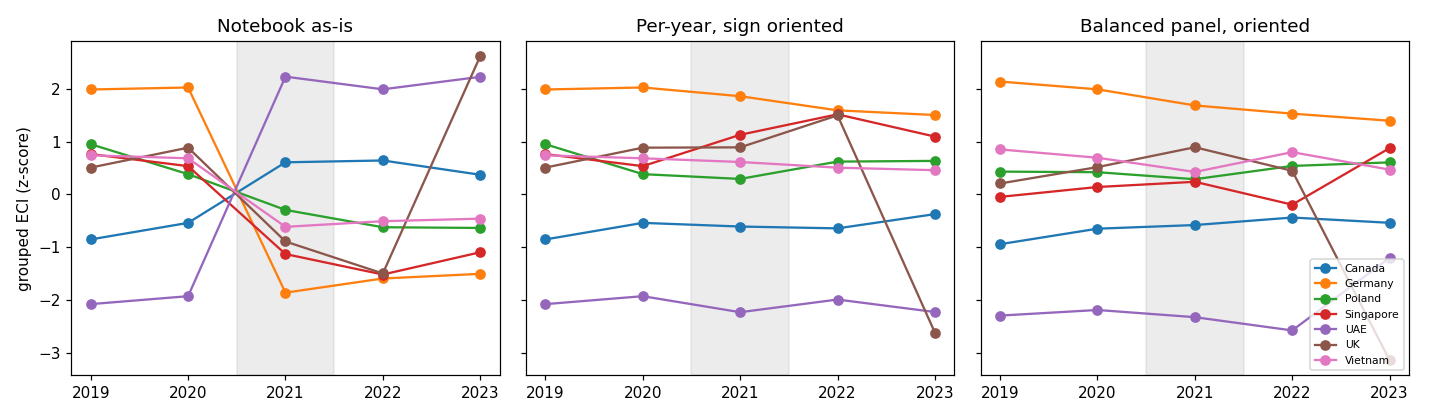
\includegraphics[width=\textwidth]{2026-11-12_Q03-fixed-panel/figures/report_country_paths.png}
\caption{Q03. Grouped ECI of the Spring 2026 report countries. The shaded 2021 drop disappears once the sign is oriented.}
\end{figure}

\textbf{Answer.} D3 is a sign artifact (consistent with Q01). Orient the sign; a fixed panel is a second-order refinement. HS4 is more stable than any grouped version (mean 0.972 vs 0.931 for 2019--2022).

\subsection{Q04: Granularity ladder}\label{sec:q04}

\emph{Metric:} $R^2$ of log GDP per capita (PPP) on ECI, same 132 countries at every level, 2019. \emph{Baseline:} the lab's 18 groups.

\begin{table}[H]\centering\small
\caption{Q04. ECI vs log GDP per capita by product granularity (2019, 132 countries unless noted).}\label{tab:q04}
\begin{tabular}{lrrrr}
\toprule
Level & Products & $R^2$ & Spearman & max $|$ECI$|$ (country) \\
\midrule
HS sections & 21 & 0.065 & 0.354 & \\
Lab 18 groups, lab rules ($n=105$) & 18 & 0.162 & 0.424 & \\
Lab 18 groups, open rules ($n=128$) & 18 & 0.154 & 0.433 & \\
Lab 18 groups rebuilt from raw & 18 & 0.173 & 0.468 & \\
HS2 & 96 & 0.328 & 0.612 & \\
\textbf{HS4} & 1224 & \textbf{0.583} & \textbf{0.784} & 2.39 (JPN) \\
HS6 & 5523 & 0.002 & 0.560 & 10.35 (GAB) \\
\midrule
Random partitions of HS6, $k=18$ (mean of 10) & 18 & 0.005 & & \\
Random partitions, $k=500$ & 500 & 0.037 & & \\
Random partitions, $k=1000$ & 1000 & 0.356 & & \\
Random partitions, $k=2000$ & 2000 & 0.488 & & \\
\bottomrule
\end{tabular}
\end{table}

\begin{figure}[H]\centering
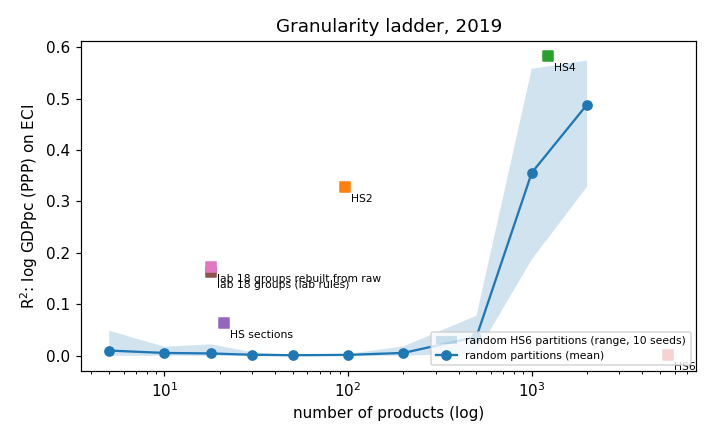
\includegraphics[width=0.7\textwidth]{2026-11-12_Q04-granularity-ladder/figures/ladder_2019.png}
\caption{Q04. $R^2$ against the number of products.}
\end{figure}

The lab's groups carry real information (a random 18-way split of HS6 gives $R^2\approx 0$), but HS4 gives 3.6 times the explained variance. HS6 is too sparse: the second eigenvector localizes on a handful of countries (Gabon 10.4 SD in 2019; Suriname 7.9 SD in 2021, where HS6 $R^2$ is 0.278). No random partition reaches 90\% of the HS4 $R^2$ even with 2000 bins, so HS4's advantage comes from its economically meaningful product boundaries, not only from the number of columns. In 2021 the ordering is the same (HS4 0.556, lab rules 0.195).

\textbf{Answer.} HS4 is the minimum level that recovers the standard ECI--income relationship. The 18-group ECI captures about a quarter of it.

\subsection{Q05: Fixing the HS-chapter mapping (D4)}\label{sec:q05}

We first rebuilt the groups from \texttt{data/raw} with the mapping in \texttt{datacleaning2025.ipynb}. The rebuild matches the cleaned CSVs exactly in 2022 and 2023 and in 77--91\% of cells in 2019--2021 (totals within 0.3\%), so in-memory remapping is a fair test. Under the current mapping chapters 84, 96 and 97 are in no regular group. Variants: \emph{fix84} adds chapter 84 to Machinery and Construction; \emph{table1} follows the Table~1 descriptions (Machinery = 84+85, Transportation = 86--89, chapter 83 to Metals, 96--97 to Daily Instruments); \emph{table1\_noagg} also drops the High-complexity aggregate.

\begin{table}[H]\centering\small
\caption{Q05. Mapping variants under lab rules, means over 2019--2022.}\label{tab:q05}
\begin{tabular}{lrrrrr}
\toprule
Variant & $\rho$ vs baseline & mean $|\Delta$rank$|$ & $R^2$ log GDPpc & $\rho$ log GDPpc & $\rho$ vs HS4 \\
\midrule
Baseline (cleaned CSV) & 1.000 & 0.0 & 0.242 & 0.524 & 0.776 \\
Rebuilt (same mapping) & 0.994 & 2.1 & 0.251 & 0.542 & 0.771 \\
fix84 & 0.966 & 5.8 & \textbf{0.283} & 0.564 & 0.785 \\
table1 & 0.948 & 6.3 & 0.277 & \textbf{0.568} & \textbf{0.789} \\
table1\_noagg & 0.934 & 8.0 & 0.203 & 0.518 & 0.776 \\
\bottomrule
\end{tabular}
\end{table}

In 2019 the fixes move the report countries substantially: Canada 108 $\rightarrow$ 89 (fix84) $\rightarrow$ 70 (table1), UK 39 $\rightarrow$ 16 $\rightarrow$ 13, Germany 1 $\rightarrow$ 2 $\rightarrow$ 6 (of 120--125). Dropping the aggregate after the fix lowers income fit, as in Q02.

\textbf{Answer.} Put chapter 84 in a regular group (either variant). It is a strict improvement on every metric; keep the aggregate until the lab moves to HS4.

\subsection{Q06: Where 2023's \$45T comes from (D1)}\label{sec:q06}

\begin{table}[H]\centering\small
\caption{Q06. Export totals, US\$ trillions.}\label{tab:q06}
\begin{tabular}{lrrrrr}
\toprule
 & 2019 & 2020 & 2021 & 2022 & 2023 \\
\midrule
Cleaned CSV, all columns & 24.87 & 23.26 & 28.68 & 30.89 & 45.30 \\
\quad of which High-complexity aggregate column & 6.92 & 6.46 & 7.57 & 8.05 & 12.66 \\
\quad of which EU-28 row & 2.89 & 2.80 & 3.29 & 3.48 & 7.11 \\
Cleaned, without aggregate and EU-28 & 16.08 & 14.98 & 18.93 & 20.54 & 28.01 \\
Raw mega, countries only & 18.43 & 17.19 & 21.71 & 23.13 & 31.52 \\
Growth Lab goods exports (all countries) & 17.29 & 16.19 & 20.33 & 22.66 & 21.66 \\
WDI world merchandise exports & 19.10 & 17.73 & 22.40 & 25.04 & 24.02 \\
\bottomrule
\end{tabular}
\end{table}

Two layers explain the \$45T. The by-design double counting (the aggregate column and the EU-28 row, which re-counts its members) accounts for the gap between 45.30 and 28.01. The remaining 28.01 is still far above 2022 (20.54) and above both external benchmarks, and the raw file shows the same jump (31.52), so the problem is in the pull, not the cleaning. Comparing each reporter's raw total with the Growth Lab: the median ratio is 1.03--1.04 in 2019--2022 and 1.18 in 2023; the number of reporters above 1.5$\times$ jumps from 3--7 to 64 of 154; 20 sit between 1.8$\times$ and 2.2$\times$ and 36 above 2.2$\times$. The largest increases 2022$\rightarrow$2023 are Germany (\$1,686B $\rightarrow$ \$4,049B; 2.58$\times$ Growth Lab), Switzerland (\$400B $\rightarrow$ \$1,669B; 4.22$\times$), Czechia (4.09$\times$), Mexico (1.96$\times$), Canada (1.98$\times$) and India (2.10$\times$). By chapter, the increase is concentrated in 87 (vehicles, +\$1,230B), 85 (+\$915B), 84 (+\$880B), 71 (+\$692B) and 30 (+\$602B). No HS6 code is duplicated within any year's file. A cluster of ratios near 2 suggests rows summed twice (for example, a partner or customs-procedure breakdown added to its own total); the larger ratios suggest more than one such breakdown.

Because RCA is a within-country share, uniform inflation of a reporter cancels; this is why 2023 HS4 ECI still agrees with the Growth Lab at Spearman 0.970 (Q13). Group \emph{levels}, growth rates and the greedy's dollar budgets are not protected.

\textbf{Answer.} A pull problem concentrated in large manufacturing exporters. Re-pull 2023 (see the data request filed with this PR).

%=====================================================================
\section{Method variants}

\subsection{Q13: Benchmark against Harvard's published ECI}\label{sec:q13}

\begin{table}[H]\centering\small
\caption{Q13. Spearman correlation with the Growth Lab's published ECI.}\label{tab:q13}
\begin{tabular}{lrrrrr}
\toprule
 & 2019 & 2020 & 2021 & 2022 & 2023 \\
\midrule
Our library on Growth Lab HS4 trade & 0.979 & 0.978 & 0.985 & 0.979 & 0.975 \\
Our library on repo Comtrade HS4 (pop $\ge$ 1M) & 0.974 & 0.975 & 0.967 & 0.970 & 0.970 \\
Lab grouped ECI, oriented & 0.687 & 0.737 & 0.770 & 0.770 & 0.717 \\
Notebook as-is & 0.687 & 0.737 & $-$0.771 & $-$0.770 & $-$0.718 \\
\bottomrule
\end{tabular}
\end{table}

Our implementation is correct: on the Growth Lab's own trade data it reproduces their ECI at 0.975--0.985 (the residual reflects their extra cleaning, e.g.\ product filters and averaging). Switching data source to our Comtrade pull costs little. The largest 2019 disagreements are commodity exporters, where our pull and the Growth Lab's mirror-reconciled data diverge most: Republic of Congo (our rank 92 vs 119), Kuwait (35 vs 58), Argentina (94 vs 71), Qatar (89 vs 67). Saudi Arabia's 2019 raw total is \$49.4B against the Growth Lab's \$188.6B, so most of its oil is missing from our pull.

\subsection{Q07: Continuous vs binary RCA}\label{sec:q07}

\emph{Metrics:} Spearman and $R^2$ with log GDP per capita, and year-to-year rank stability, means over 2019--2022. \emph{Baseline:} binary RCA $\ge 1$.

\begin{table}[H]\centering\small
\caption{Q07. RCA variants at HS4.}\label{tab:q07}
\begin{tabular}{lrrrrrr}
\toprule
 & \multicolumn{3}{c}{Repo Comtrade HS4} & \multicolumn{3}{c}{Growth Lab HS4} \\
\cmidrule(lr){2-4}\cmidrule(lr){5-7}
Variant & $\rho$ inc. & $R^2$ inc. & stability & $\rho$ inc. & $R^2$ inc. & stability \\
\midrule
Binary RCA $\ge$ 1 & 0.783 & 0.581 & 0.972 & 0.812 & 0.627 & 0.981 \\
$\log(1+\text{RCA})$ & 0.784 & 0.583 & \textbf{0.983} & 0.816 & 0.639 & \textbf{0.994} \\
$\min(\text{RCA}, 2)$ & \textbf{0.794} & \textbf{0.605} & 0.975 & 0.813 & 0.635 & 0.991 \\
RCA percentile within product & 0.734 & 0.450 & 0.982 & \textbf{0.831} & \textbf{0.646} & 0.990 \\
\bottomrule
\end{tabular}
\end{table}

Continuous RCA is slightly more stable and fits income about as well; the ranking barely moves (Spearman with binary 0.987 for log RCA, 0.992 for capped). No variant wins consistently across the two data sources. In the out-of-time growth test (Q16) $\log(1+\text{RCA})$ does worse than binary ($-5.7\%$ vs $-1.8\%$ out-of-sample $R^2$).

\textbf{Answer.} Continuous RCA is a reasonable robustness check, not an upgrade. Keep binary as the headline.

\subsection{Q08: Fitness-Complexity}\label{sec:q08}

\begin{table}[H]\centering\small
\caption{Q08. Fitness vs ECI at HS4 (means over 2019--2022).}\label{tab:q08}
\begin{tabular}{lrrrrrr}
\toprule
 & \multicolumn{3}{c}{Repo Comtrade HS4} & \multicolumn{3}{c}{Growth Lab HS4} \\
\cmidrule(lr){2-4}\cmidrule(lr){5-7}
Measure & $\rho$ inc. & $R^2$ inc. & stability & $\rho$ inc. & $R^2$ inc. & stability \\
\midrule
ECI (binary) & 0.783 & 0.581 & 0.972 & 0.812 & 0.627 & 0.981 \\
log Fitness & 0.473 & 0.084 & 0.982 & 0.607 & 0.069 & 0.988 \\
Diversity & 0.359 & 0.151 & 0.983 & 0.513 & 0.252 & 0.989 \\
\bottomrule
\end{tabular}
\end{table}

Fitness and ECI agree on rank (Spearman 0.827 on repo data, 0.895 on Growth Lab data; mean absolute rank difference 16.7 and 14.0 places in 2019) but Fitness tracks income much less. Its log values for the weakest exporters keep falling with more iterations (Pearson $R^2$ with income falls from 0.153 at 10 iterations to 0.081 at 200) while the rank correlation is fixed at 0.506 from 20 iterations on, so only ranks should be compared. The largest disagreements are small rich economies with narrow baskets, which Fitness penalizes: Brunei (ECI rank 29, Fitness rank 126), Kuwait (39 vs 123), Malta (20 vs 81), Ireland (17 vs 62). India moves the other way (52 vs 15). Fitness was the least-bad complexity variant out of time (Q16: $-0.56\%$), but it still did not beat the baseline.

\begin{figure}[H]\centering
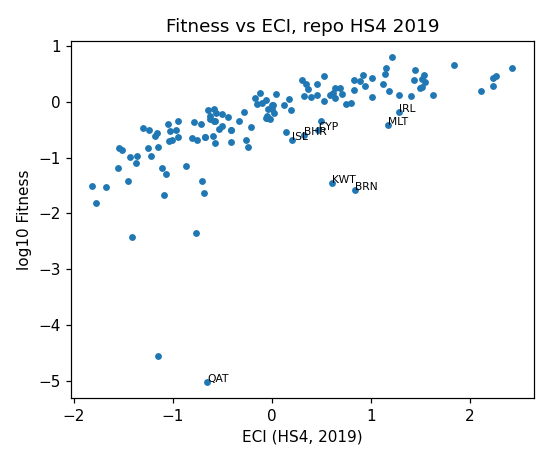
\includegraphics[width=0.5\textwidth]{2026-11-12_Q08-fitness-complexity/figures/fitness_vs_eci_2019.png}
\caption{Q08. Fitness vs ECI, repo HS4, 2019.}
\end{figure}

\subsection{Q09: How fragile are ECI ranks?}\label{sec:q09}

\emph{Metrics:} median width of each country's 90\% rank interval under 300 product-bootstrap draws (as a share of the number of countries); mean $|\Delta$rank$|$ when one country is left out (LOCO); eigengap $\lambda_2-\lambda_3$ of $\tilde M_{cc'}$.

\begin{table}[H]\centering\small
\caption{Q09. Rank fragility, 2019.}\label{tab:q09}
\begin{tabular}{lrr}
\toprule
 & Grouped (18, lab rules) & HS4 (repo) \\
\midrule
Countries & 121 & 133 \\
Median 90\% interval width (share of ranking) & 0.680 & 0.196 \\
Mean 90\% interval width (ranks) & 84.6 & 28.6 \\
Share of countries with interval wider than a quarter of the ranking & 1.00 & 0.26 \\
LOCO mean $|\Delta$rank$|$ (worst single drop) & 1.24 (5.68) & 0.61 (2.48) \\
\midrule
Germany: rank [90\% interval] & 2 [1.5, 55] & 6 [4, 7] \\
UK & 41 [5, 110] & 14 [8, 18] \\
Canada & 93 [28, 106] & 45 [31, 60] \\
Singapore & 31 [6, 103] & 5 [2, 6] \\
\bottomrule
\end{tabular}
\end{table}

The eigengap does not separate the two (grouped 0.069--0.125, HS4 0.078--0.094 across 2019--2023; Growth Lab HS4 0.076--0.085), so a small gap is not the problem. The problem is that with 18 columns a country's ranking hinges on a few binary RCA cells; resampling which groups are present reshuffles almost everyone. Removing a single country matters less.

\begin{figure}[H]\centering
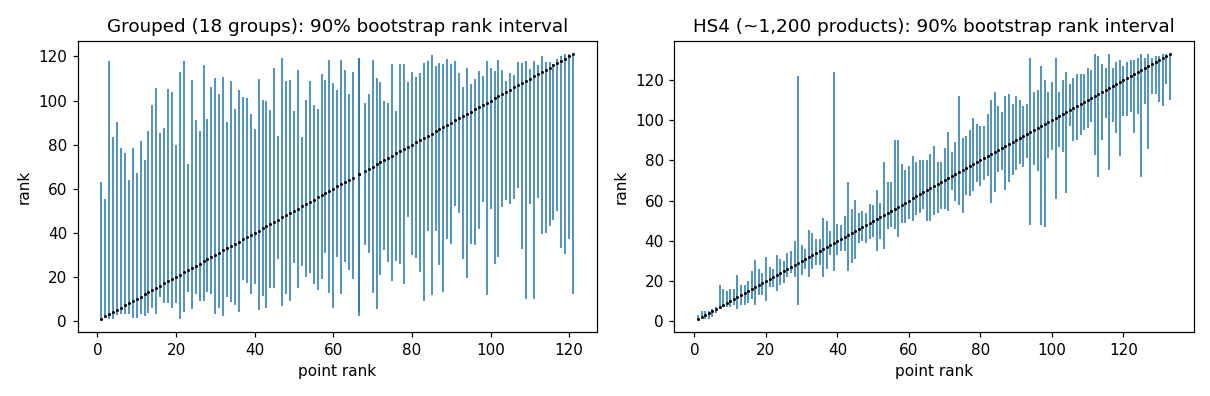
\includegraphics[width=\textwidth]{2026-11-12_Q09-rank-fragility/figures/rank_intervals_2019.png}
\caption{Q09. 90\% bootstrap rank intervals, grouped vs HS4.}
\end{figure}

\textbf{Answer.} Grouped ECI ranks are too uncertain to support statements like ``Canada ranks 93rd''. HS4 ranks are precise to a few places for most countries.

\subsection{Q15: Population-adjusted RCA}\label{sec:q15}

We define per-capita RCA as $\text{RpcA}_{cp} = (x_{cp}/\text{pop}_c)/(\sum_c x_{cp}/\sum_c \text{pop}_c)$ and compare $M=\mathbb 1[\text{RCA}\ge1]$, $M=\mathbb 1[\text{RpcA}\ge1]$ and their intersection (Growth Lab HS4, means over 2019--2022).

\begin{table}[H]\centering\small
\caption{Q15. Per-capita RCA variants.}\label{tab:q15}
\begin{tabular}{lrrrrrr}
\toprule
Variant & $\rho$ inc. & $R^2$ inc. & stability & $\rho$ vs published & growth coef/SD ($p$) & $\Delta R^2$ \\
\midrule
RCA $\ge$ 1 & 0.812 & 0.627 & 0.981 & 0.980 & 0.566 (0.015) & 0.014 \\
RpcA $\ge$ 1 & 0.836 & 0.580 & 0.986 & 0.923 & 0.341 (0.198) & 0.006 \\
RCA $\ge$ 1 and RpcA $\ge$ 1 & \textbf{0.855} & \textbf{0.688} & 0.986 & 0.934 & 0.284 (0.316) & 0.003 \\
\bottomrule
\end{tabular}
\end{table}

On repo data (2019, 126 countries) the same pattern holds: income $R^2$ 0.585 (RCA), 0.677 (RpcA), 0.736 (both). Per-capita adjustment fits income better because exports per person are themselves close to income, and it adds nothing to growth prediction: with both in the 10-year growth regression the RCA version keeps its coefficient (0.493, $p=0.023$) and the RpcA version does not (0.181, $p=0.476$). It mainly demotes large, poor countries (India 49th $\rightarrow$ 104th, Philippines 33rd $\rightarrow$ 83rd) and promotes small ones (Bangladesh 111th $\rightarrow$ 64th).

\textbf{Answer.} Not worth adopting. Better income fit here is partly mechanical.

\subsection{Q11: Does the greedy optimizer's target change under HS4 ECI?}\label{sec:q11}

For each Spring 2026 country and group we added 5\% of the country's total exports to that group and recomputed its ECI. On the HS4 side the bump is spread over the group's HS4 products in proportion to the country's exports there (Services has no HS4 counterpart and is excluded from the comparison).

\begin{table}[H]\centering\small
\caption{Q11. Best group for a 5\% export bump, 2022 (the notebook's greedy year).}\label{tab:q11}
\begin{tabular}{llll}
\toprule
Country & Grouped ECI (excl.\ Services) & HS4 ECI & Spearman of gain rankings \\
\midrule
Canada & Daily Instruments & Daily Instruments & 0.450 \\
Germany & Weapons & Daily Instruments & 0.628 \\
Poland & High-complexity Products & Chemicals & 0.132 \\
Singapore & High-complexity Products & Daily Instruments & 0.598 \\
UAE & Daily Instruments & Chemicals & 0.258 \\
UK & Daily Instruments & Daily Instruments & 0.654 \\
Vietnam & Machinery and Construction & Metals & 0.142 \\
\bottomrule
\end{tabular}
\end{table}

The best group agrees for 2 of 7 countries in 2022 and 0 of 7 in 2019 (mean Spearman between the two gain rankings 0.409 and 0.528). Including Services, the grouped ECI's best target in 2022 is Services for 3 countries and the High-complexity aggregate for 2 more, so the optimizer is drawn to the non-goods and circular columns. HS4 ECI favors Chemicals and Daily Instruments (precision instruments).

\emph{Sign check (proposal 2026-11-11 \#1):} across 126 single-group perturbations per year the notebook's sign never flips relative to the unperturbed matrix. But in 2022 the unperturbed sign is itself reversed (anti-correlated with diversity), so every comparison the optimizer makes in 2022 ranks allocations by \emph{lower} complexity. The same holds for 2021 and 2023 per Q01.

\textbf{Answer.} Yes, the target changes for most countries. Any greedy result on 2021--2023 grouped data should be treated as invalid until the sign is fixed.

%=====================================================================
\section{Does complexity predict growth?}

\subsection{Q10: The 2019--2023 window}\label{sec:q10}

Outcome: annualized growth of real GDP per capita, 2019--2023 (WDI constant US\$; PPP gives the same picture). Baseline: log GDP per capita 2019 plus the resource export share, $R^2=0.012$, 132 countries. Adding any 2019 score, one at a time, changes $R^2$ by at most 0.007 and no coefficient is significant: HS4 ECI $-0.106$ per SD ($p=0.762$), log RCA ECI $-0.026$ ($p=0.926$), log Fitness 0.338 ($p=0.214$), diversity 0.026 ($p=0.917$), entropy $-0.038$ ($p=0.929$), Growth Lab ECI 0.608 ($p=0.083$), and the lab's grouped ECI $-0.019$ ($p=0.945$, 105 countries). Trimming the 5\% most extreme growth rates (largest: Guyana, Lebanon, Georgia, Myanmar, Albania) does not help (HS4 ECI 0.183, $p=0.430$).

\textbf{Answer.} Null, as expected for a four-year window that contains COVID and the 2022 commodity shock. The reports' 5-year comparisons should not be read as tests of ECI.

\subsection{Q12: Replicating the Atlas 10-year regression}\label{sec:q12}

Design: annualized growth over 1995--2005, 2004--2014 and 2013--2023 on initial ECI (standardized within window), log initial GDP per capita, resource rents (\% GDP), resource export share and window fixed effects; HC1 standard errors. 358 observations, 141 countries.

\begin{table}[H]\centering\small
\caption{Q12. 10-year growth regressions (coefficients per SD of the added score).}\label{tab:q12}
\begin{tabular}{lrrrr}
\toprule
Added to baseline & coef (SE) & $p$ & $R^2$ & $\Delta R^2$ \\
\midrule
Baseline (income + resources + window FE) & & & 0.196 & \\
Growth Lab published ECI & 0.749 (0.244) & 0.002 & 0.222 & 0.026 \\
Our ECI on Growth Lab HS4 & 0.566 (0.234) & 0.015 & 0.210 & 0.014 \\
Export entropy & 0.653 (0.244) & 0.007 & 0.211 & 0.015 \\
Diversity & 0.196 (0.178) & 0.271 & 0.199 & 0.003 \\
\midrule
PPP outcome: Growth Lab ECI & 0.941 (0.268) & $<0.001$ & 0.217 & 0.038 \\
PWT outcome, 1995--2005 and 2005--2015 ($n=215$) & 0.204 (0.341) & 0.549 & 0.125 & 0.003 \\
\bottomrule
\end{tabular}
\end{table}

\begin{table}[H]\centering\small
\caption{Q12. The ECI coefficient by window (cross-sections).}\label{tab:q12b}
\begin{tabular}{lrrrrr}
\toprule
Window & $n$ & coef/SD & $p$ & $R^2$ baseline & $R^2$ with ECI \\
\midrule
1995--2005 & 100 & 0.892 & 0.016 & 0.110 & 0.156 \\
2004--2014 & 119 & 0.588 & 0.154 & 0.216 & 0.232 \\
2013--2023 & 139 & 0.441 & 0.333 & 0.273 & 0.281 \\
\bottomrule
\end{tabular}
\end{table}

The headline result replicates with WDI data: conditional on income, a one-SD higher ECI goes with 0.75 percentage points faster annual growth over the next decade. Without resource controls, adding ECI to income alone raises $R^2$ from 0.094 to 0.202. Three qualifications matter. (1) The effect weakens every decade and is not significant in either of the last two windows on its own. (2) With PWT real GDP over the two windows PWT covers, it disappears. (3) Within countries (5-year windows 1995--2020, country and period fixed effects, 595 observations, 139 countries, clustered SEs), the coefficient is similar (1.053) but imprecise ($p=0.077$); pooled it is 0.994 ($p<0.001$). The Growth Lab's published ECI predicts better than our recomputation on their data, plausibly because of their additional cleaning.

\begin{figure}[H]\centering
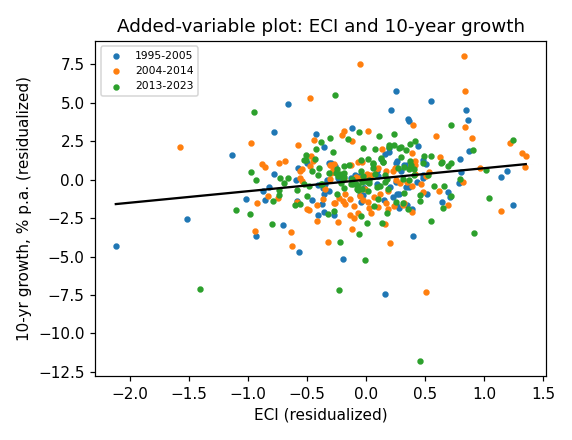
\includegraphics[width=0.55\textwidth]{2026-11-12_Q12-atlas-growth-regression/figures/added_variable.png}
\caption{Q12. Added-variable plot: residualized 10-year growth against residualized ECI.}
\end{figure}

\subsection{Q14: Mediation by capabilities}\label{sec:q14}

Same design as Q12, on one common sample of 323 observations (126 countries) with PWT human capital and WGI governance at the window start.

\begin{table}[H]\centering\small
\caption{Q14. Growth Lab ECI coefficient as capability controls are added.}\label{tab:q14}
\begin{tabular}{lrrrr}
\toprule
Model & ECI coef/SD & $p$ & share of first row & $R^2$ \\
\midrule
ECI + income + resources & 0.494 & 0.038 & 1.00 & 0.194 \\
+ human capital (log PWT hc) & 0.291 & 0.218 & 0.59 & 0.213 \\
+ governance (WGI effectiveness, rule of law) & 0.475 & 0.044 & 0.96 & 0.205 \\
+ human capital + governance & 0.252 & 0.280 & 0.51 & 0.227 \\
\midrule
Infrastructure sample ($n=246$): base & 0.414 & 0.135 & 1.00 & 0.147 \\
\quad + capabilities + internet + private credit & 0.265 & 0.307 & 0.64 & 0.177 \\
R\&D sample ($n=146$): base & 0.676 & 0.063 & 1.00 & 0.221 \\
\quad + R\&D (\% GDP) & 0.731 & 0.045 & 1.08 & 0.222 \\
\quad + R\&D + human capital & 0.567 & 0.126 & 0.84 & 0.229 \\
\bottomrule
\end{tabular}
\end{table}

Human capital, not governance or R\&D, absorbs ECI's predictive power. Without ECI, human capital predicts growth strongly (0.677 per SD, $p<0.001$) while governance is marginal (0.848, $p=0.073$). Our own recomputed ECI is not significant on this sample even before controls (0.211, $p=0.346$) and turns negative once human capital is added. In the 2013 cross-section, human capital and governance explain 75\% of the variance of ECI (126 countries), income alone 59.7\%, and adding resources reaches 82.2\%.

\textbf{Answer.} ECI largely summarizes schooling-related capabilities. About half of its growth signal survives the human-capital control, and that remainder is not statistically distinguishable from zero.

\subsection{Q16: Rolling-origin out-of-time evaluation}\label{sec:q16}

Pre-registered protocol: outcome is 10-year growth from origin $t$; baseline is pooled OLS on log income, resource rents and resource export share; each candidate adds one score. For each test origin $T=2005,\dots,2014$ the model is fit on origins $t\le T-10$ only (outcomes known by $T$). Metric: out-of-sample $R^2$ relative to the baseline, $1-\text{SSE}_\text{cand}/\text{SSE}_\text{base}$, pooled over 1,324 test observations (143 countries). The baseline itself beats a historical-mean forecast by 15.6\%.

\begin{table}[H]\centering\small
\caption{Q16. Out-of-time performance relative to the income + resources baseline. Negative = worse.}\label{tab:q16}
\begin{tabular}{lrrrr}
\toprule
Score & Rolling $R^2_\text{oos}$ & folds better & Single split $R^2_\text{oos}$ & In-sample $\Delta R^2$ \\
\midrule
log Fitness & $-0.56\%$ & 1/10 & $-0.05\%$ & 0.0020 \\
ECI, binary (ours) & $-1.82\%$ & 2/10 & $-1.20\%$ & 0.0112 \\
Diversity & $-2.31\%$ & 0/10 & $-2.11\%$ & 0.0008 \\
ECI, capped RCA & $-3.71\%$ & 3/10 & $-3.46\%$ & 0.0154 \\
ECI, RCA percentile & $-3.93\%$ & 3/10 & $-3.47\%$ & 0.0036 \\
ECI, RpcA & $-4.32\%$ & 1/10 & $-4.28\%$ & 0.0019 \\
COI (Growth Lab) & $-4.67\%$ & 0/10 & $-4.15\%$ & 0.0032 \\
ECI, RCA and RpcA & $-5.47\%$ & 1/10 & $-4.03\%$ & 0.0019 \\
ECI, $\log(1+\text{RCA})$ & $-5.69\%$ & 3/10 & $-4.71\%$ & 0.0210 \\
Export entropy & $-6.29\%$ & 1/10 & $-6.36\%$ & 0.0063 \\
ECI, Growth Lab published & $-6.98\%$ & 2/10 & $-6.53\%$ & 0.0126 \\
\bottomrule
\end{tabular}
\end{table}

Every variant improves the in-sample fit and every variant makes out-of-time forecasts worse. Dropping commodity exporters (resource share above 50\%) does not rescue any of them (binary ECI $-7.6\%$, published ECI $-13.6\%$). The likely mechanism is the same as in Q12: the ECI--growth slope estimated on the 1990s does not hold in the 2000s and 2010s, so a model that uses it extrapolates a relationship that has weakened.

\begin{figure}[H]\centering
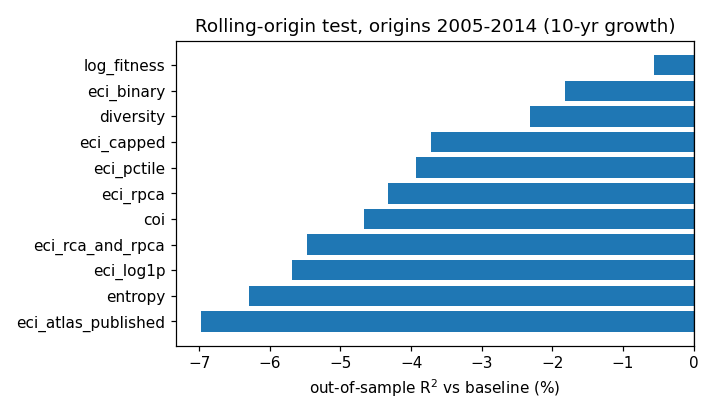
\includegraphics[width=0.65\textwidth]{2026-11-12_Q16-rolling-origin/figures/rolling_r2oos.png}
\caption{Q16. Out-of-sample $R^2$ relative to the baseline, rolling origins 2005--2014.}
\end{figure}

\textbf{Answer.} Under an honest out-of-time protocol, no ECI variant (including the Growth Lab's) beats income plus natural resources at forecasting 10-year growth for origins 2005--2014. This is the strongest evidence in this paper against using ECI as an optimization target.

%=====================================================================
\section{Implications for the lab}

\paragraph{Measurement fixes (do now).}
\begin{enumerate}
\item \textbf{Orient the ECI sign} in \texttt{compute\_eci} (one line: flip if it correlates negatively with diversity). Without this, 2021--2023 ECI levels, changes, peer comparisons and greedy results are reversed.
\item \textbf{Compute ECI at HS4} from \texttt{data/raw} with \texttt{lib/eci.py}, and use the 18 groups only to present results. This raises income $R^2$ from 0.16 to 0.58, narrows rank intervals from 68\% to 20\% of the ranking, and brings agreement with Harvard's ECI from 0.69--0.77 to 0.97.
\item If the groups stay in the pipeline: \textbf{put HS 84 in a regular group} (Q05), drop the EU-28 row, and stop letting Services and the High-complexity aggregate drive the optimizer (Q11).
\item \textbf{Re-pull 2023} and add a reconciliation check against the Growth Lab or WDI totals to the data-update workflow (Q06).
\end{enumerate}

\paragraph{Interpretation (change how reports talk about ECI).}
\begin{enumerate}
\item ECI is a good description of how similar a country's export basket is to rich countries' baskets, and it predicted 10-year growth in the 1995--2005 cross-section. That relationship has weakened since, is mostly shared with human capital, and does not survive an out-of-time test.
\item The greedy optimizer's premise (raise ECI $\Rightarrow$ raise growth) is therefore not supported by our evidence. Reports should present the allocation as ``which export moves would make the basket look most like high-complexity economies'', not as a growth strategy.
\item Do not attach growth interpretations to 5-year ECI changes (Q10).
\end{enumerate}

\paragraph{Variants not worth adopting.} Continuous RCA (Q07), Fitness (Q08) and per-capita RCA (Q15) each win on some descriptive metric, but none improves out-of-time prediction. Keep binary HS4 ECI as the standard and the others as robustness checks.

%=====================================================================
\section{Limitations}
\begin{itemize}
\item Growth tests have three non-overlapping 10-year windows; the rolling test reuses overlapping windows in training, and its early folds train on a single origin year (about 100 countries).
\item Our long-panel complexity scores are computed from the Growth Lab's trade data, not our Comtrade pull, which covers only 2019--2023.
\item GDP per capita comes from WDI (constant 2015 US\$); the PWT robustness check ends in 2019 and disagrees.
\item Q11 measures one-step marginal gains, not the full two-step greedy (which we did not run, per the protocol).
\item The 2023 diagnosis identifies \emph{which} reporters and chapters are inflated, not the exact pull parameter that caused it; that needs the original Comtrade query.
\item The mediation results are associations; human capital is itself endogenous to growth.
\end{itemize}

%=====================================================================
\section*{Reproducibility}
Every result is regenerated by \texttt{willbetts/nightly/run\_all.sh}, which fetches the external data (\texttt{external-data/scripts/}), builds the score panel, and runs \texttt{runs/2026-11-12\_Q*/run.py}. Each run folder holds its script, \texttt{results.json} and \texttt{figures/}. Shared code: \texttt{lib/eci.py} (Q01; this run adds Italy's Comtrade code) and \texttt{lib/research.py} (new).

\section*{References}
\small
\begin{itemize}[leftmargin=*,label={}]
\item Feenstra, R. C., Inklaar, R., \& Timmer, M. P. (2015). The next generation of the Penn World Table. \emph{American Economic Review} 105(10).
\item Hausmann, R., Hidalgo, C. A., et al. (2013). \emph{The Atlas of Economic Complexity}. MIT Press.
\item Hidalgo, C. A., \& Hausmann, R. (2009). The building blocks of economic complexity. \emph{PNAS} 106(26).
\item Kaufmann, D., Kraay, A., \& Mastruzzi, M. (2010). The Worldwide Governance Indicators: methodology and analytical issues. World Bank Policy Research Working Paper 5430.
\item Mealy, P., Farmer, J. D., \& Teytelboym, A. (2019). Interpreting economic complexity. \emph{Science Advances} 5(1).
\item Tacchella, A., Cristelli, M., Caldarelli, G., Gabrielli, A., \& Pietronero, L. (2012). A new metrics for countries' fitness and products' complexity. \emph{Scientific Reports} 2.
\item The Growth Lab at Harvard University (2025). International Trade Data (HS92). Harvard Dataverse, doi:10.7910/DVN/T4CHWJ.
\item World Bank. World Development Indicators (bulk download, accessed 2026-11-12).
\end{itemize}

\end{document}
